% Chapter 4
\chapter{Results and conclusion} % Write in your own chapter title
\label{Chapter4}
\indent We have surveyed previous work done in similar domain in chapter
~\ref{Chapter1}. We have discussed different background subtraction and
human detection techniques in chapter ~\ref{Chapter2}. We have also
discussed about technique used for human detection in our work in the
same chapter.  Since we have used \textbf{Skel}etonized \textbf{Mot}ion
analysis for human detection, therefore we name our technique as
SKELMOT. We have talked about embedded implementation of our work in
chapter~\ref{Chapter3}. In this section we discuss results of different
evaluations and also how does SKELMOT compares with others. We also draw
conclusions from our results and future works to be done.
\section{Results}
\indent We did comparison of execution time of background subtraction
algorithm in Fig.~\ref{bg_compare}. Graph shows that Vibe is far more
computationally efficient compared to other. Therefore we used Vibe
algorithm in our implementation, where we target human detection based
on its skeleton motion. Vibe has lower computation requirement even
while maintaining excellent results because of following reasons:
\begin{itemize}
	\item It does not save complete frame as background sample,
		rather it chooses random samples for replacement. But it
		insures that the sample lifespan decays exponentially.
	\item Samples corresponding to neighbouring pixel is updated
		again on random basis.
	\item Model is initialized with first frame itself, therefore first
		background subtracted object is obtained as early as
		second frame.
\end{itemize}
\indent We have seen different skeleton output in Fig.~\ref{skeletons}.
Skeleton obtained by morphological method is discontinuous. Hough
transform can be used to connect these unconnected skeleton points.
Further morphological operations can be used to find skeleton endpoints.
On top of it, some heuristic need to be used for detection of skeleton
endpoints corresponding to legs end. These all operations are
computationally expensive. Skeleton obtained by distance transform
method has also similar issues.\\
\indent Contour method provides outer boundary of the moving object. If
a detection method is based on shape, then uses of contour might give
good result. But we have targeted human detection using leg motion
analysis for a simple reason that, it provides reasonably good
results(under some limitations) even with low end CPUs. Therefore we
processed contour further to get star skeleton. We have seen that
finding a star skeleton is very simple in nature.
\begin{figure}[!t]
\centering
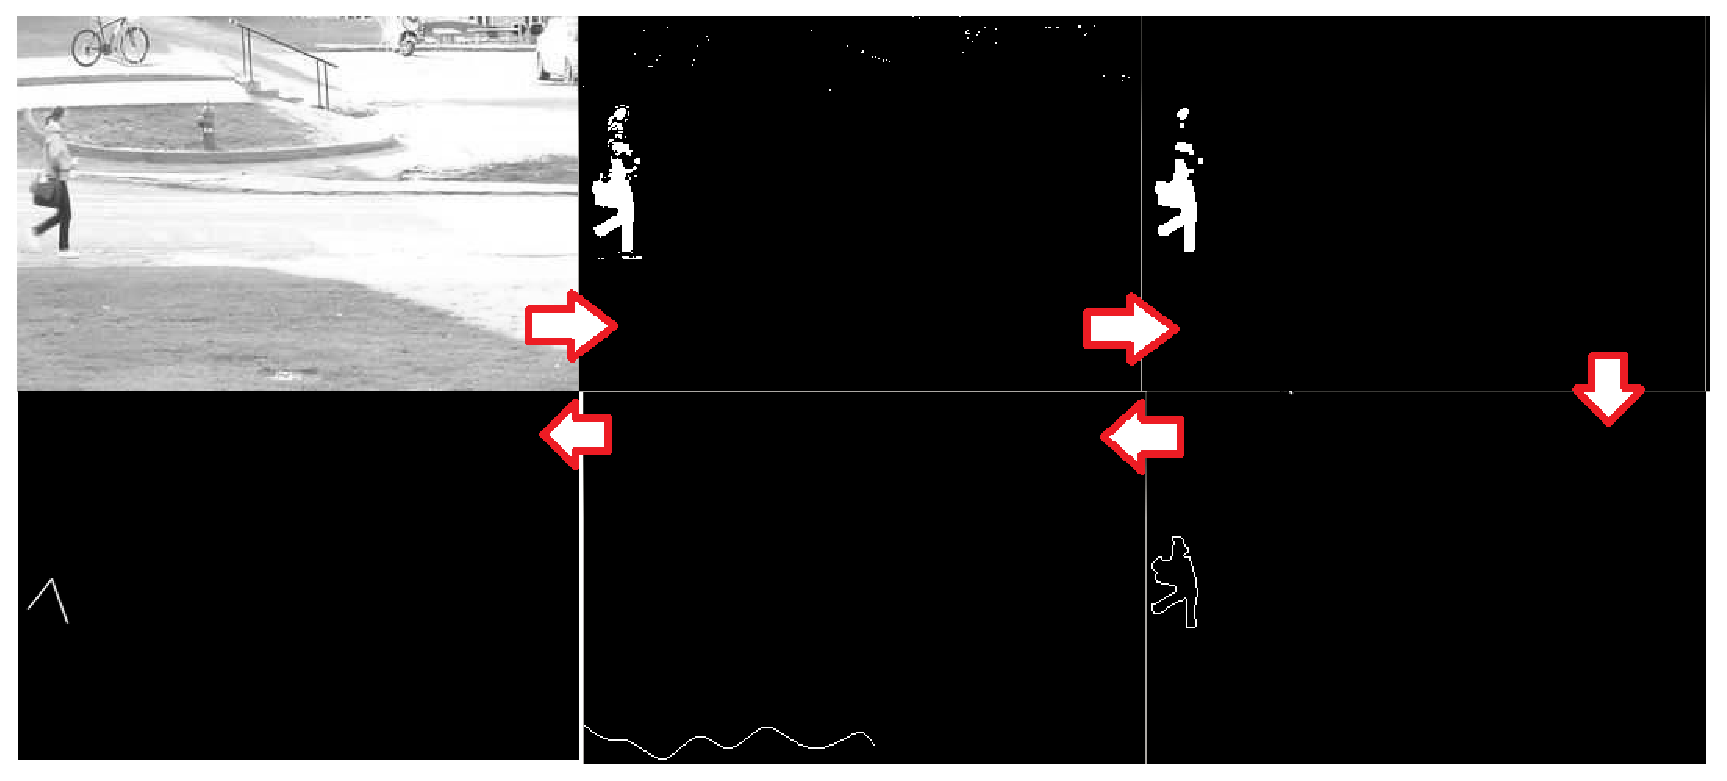
\includegraphics[height=200pt]{Figures/pipeline_images}
\caption{Images at different stages of processing. (From top left in
	clockwise order)\\
	\textbf{(a)} Gray Scale input frame\\
	\textbf{(b)} Foreground extracted image using Vibe\\
	\textbf{(c)} Cleaned image\\
	\textbf{(d)} Contour of moving object\\
	\textbf{(e)} Plot of three points of interest, centroid and two distance
peaks nearer to bottom left and bottom right corner of bounding box\\
\textbf{(f)} Virtual representation of scene} 
\label{pipeline_images}
\end{figure}
\begin{figure}[!b]
\centering
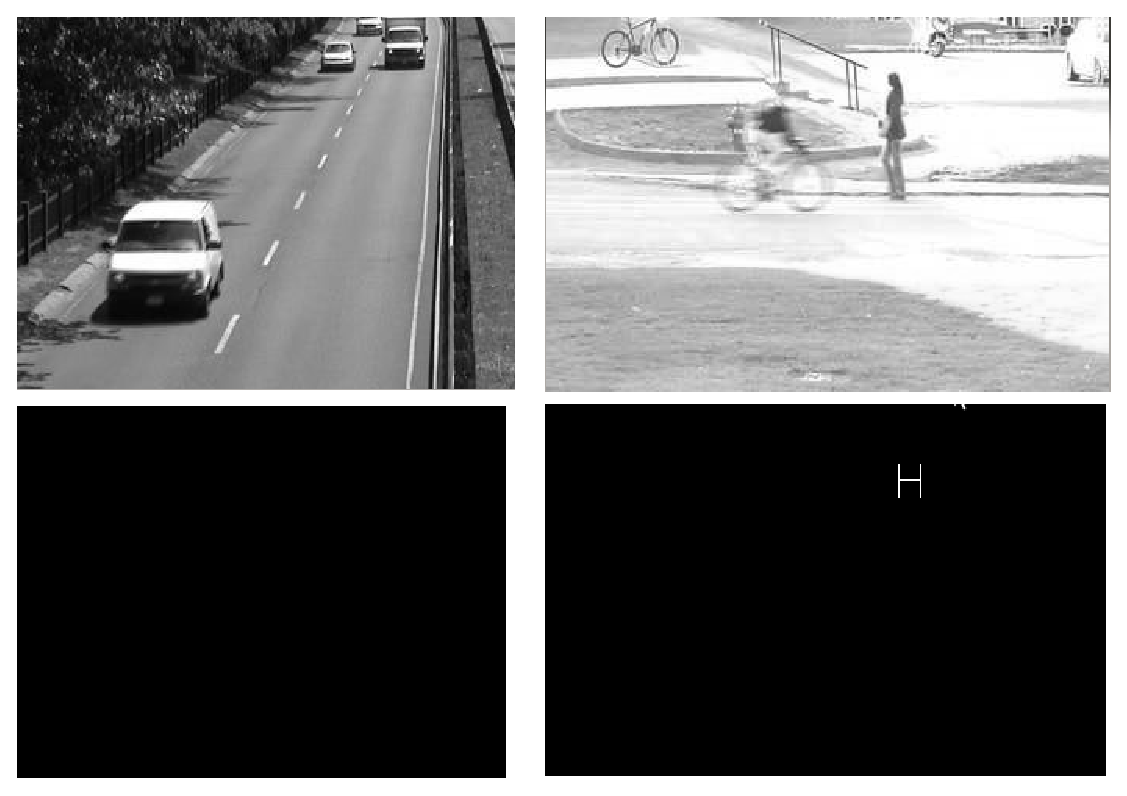
\includegraphics[height=220pt]{Figures/negative_inputs}
\caption{Input and output in case of negative images}
\label{negative_inputs}
\end{figure}

\indent We took input video dataset from www.changedetection.net
~\cite{36}. This website is maintaining benchmarking results for
algorithms related to change and motion detection. Fig.~\ref{pipeline_images} shows
output images at different stages of processing.\\
\indent We have used SKELMOT with two surveillance video from the above
website. First test video consists of frames having pedestrian with
different speed and a person moving on bicycle. We conclude that with
SKELMOT, system is able to detect all moving pedestrians after its three
steps move. We have seen that it successfully rejects a person moving on
bicycle and does not recognize him as true object. We took a highway
surveillance video having frames of moving vehicles. We used SKELMOT to
detect and recognize moving objects. We conclude that SKELMOT is
successfully able to discriminate and does not recognize them as human.
Fig.\ref{negative_inputs} shows how it rejects moving vehicle and
bicycle and does not detect them as human.\\
\indent We have implemented and executed SKELMOT, Haar-like~\cite{19} and
covariance~\cite{19} feature based detection algorithm on both x86
desktop computer and embedded ARM platform. We did benchmarking of both
systems using "BYTE Unix Benchmarks Dhrystone" version 3.6 code. This benchmarking
provides a index for the comparison of unix like systems. Dhrystone is
very useful in measurement and comparison of CPU performances. X86 based
Linux PC was measured as DMIPS = 800, while ARM CPU was measured as
DMIPS = 44.\\
\begin{figure}[!b]
\centering
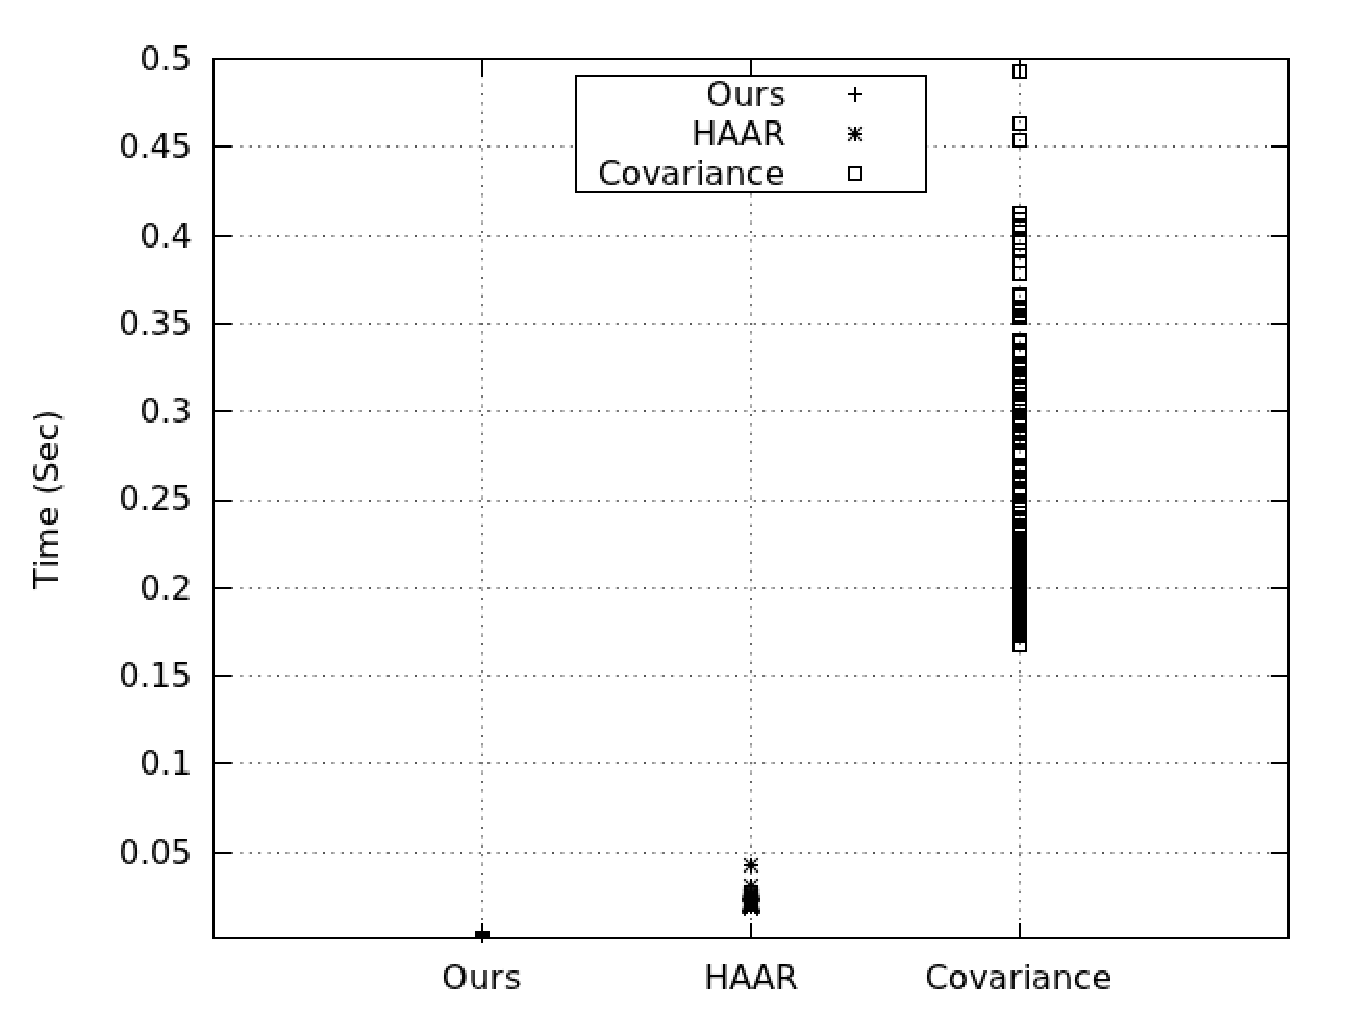
\includegraphics[scale=0.60]{Figures/pipeline_execution_time}
\caption{Execution time of evaluated algorithms on ARM and x86
platform}
\label{pipeline_execution_time}
\end{figure}
\indent Fig.\ref{pipeline_execution_time} shows comparison of execution
time for different algorithms at both x86 as well as at ARM platform. We
can see that there is definite improvement in execution speed of SKELMOT
over HAAR and covariance feature based approach. SKELMOT takes just 3.6
ms on the average, while HAAR and covariance feature based algorithm
take around 20 ms and 248 ms respectively per frame on x86 platform.
Comparison of timing on ARM platform shows that SKELMOT takes 182 ms on
the average, while HAAR and covariance feature based algorithm take
around 942 ms and 4.65 s respectively per frame. Therefore, we conclude
that SKELMOT detects human at the rate of at least five frames per second
even with ARMV6 CPU platform.
\section{Conclusion}
\indent We can draw following conclusion on the basis of result obtained 
in previous section.
\begin{itemize}
	\item 	We have seen that method based on covariance or
		Haar-like descriptor is very slow in comparison with
		skeleton motion descriptor. When these algorithms are
		implemented with low end embedded CPUs then, a
		pedestrian detector based on Haar-like features detects
		at the rate of almost one frame per second. A pedestrian
		detector based on covariance feature detects at the rate
		of almost one frame per five seconds. Such algorithms
		are not suitable for low cost embedded CPUs. However, if
		we still wish to use these algorithms for human
		detection then, we will need to implement them using
		dedicated hardware accelerator.
	\item 	Many surveillance applications like detection of moving
		person at a traffic light or in an indoor corridor will
		not need to use complex algorithms. It can work well with
		simple algorithms like leg motion analysis. In such cases
		human would be moving with reasonably same speed. Therefore,
		for such applications we do not need to use complex algorithm
		to get real time performance with low cost embedded platform.
		By using proposed algorithm SKELMOT, we can save a lot of
		computational power.
\end{itemize}
\section{Future work}
Future work may be carried in following directions:
\begin{itemize}
\item Test of this algorithm with real camera connected and Zigbee
network will provide good confidence to use it.
\item A research work may be initiated to see actual power saving using
such a low complexity algorithm.
\item There can be improvement in blob tracking algorithm to predict
next position on the basis of past N number of frames.
\item We have seen that low end micro-controller is not able to work with
single frame human detection algorithms. These algorithm can either run on
high performance CPU, or GPU. A work can be initiated to implement such
algorithms in hardware and then to use this hardware with low end
micro-controller. It would be interesting to see difference between power
consumption of two systems ie one when complex algorithms have been
implemented using high performance CPU/GPU or, with a low performance
CPU and dedicated hardware accelerator.
\end{itemize}

